\documentclass[10pt]{article}
\usepackage[portuguese]{babel}
\usepackage[utf8]{inputenc}
\usepackage[pdftex]{graphicx}
\usepackage{venndiagram}
\usepackage{subcaption}
\usepackage{caption}
\usepackage[backend=biber,style=authoryear-ibid]{biblatex}
\usepackage[normalem]{ulem}
\usepackage[margin=0.8in]{geometry}
%\addbibresource{}
\graphicspath{{Pictures/}}
\usepackage{tikz}
\usepackage{setspace}
\usepackage{enumitem}
\usepackage{textcomp}
\usepackage{listings}
\usepackage{float}


\author{}
\title{}
\date{}

\newcommand{\quotebox}[3]{
  \begin{center}
\noindent\fbox{ 
  \parbox{#3\textwidth}{%
  {\itshape#1\itshape}

  \raggedleft {\textbf{#2}} 
    }%  
}
\end{center}
}

\newcommand{\spawnfig}[3]
{
  \begin{figure}[h]
  \centering
  \includegraphics[scale={#3}]{#1}
  \caption{#2}
  \end{figure}
}


\begin{document}
\maketitle

\section{Program Scope}

The program should be able to receive as input a chess move in UCI(Universal
Chess Interface) format i.e
e2e4, and if the movement is valid, output the board state to the user or inform
the user the input isn't valid. For this matter, the standard python library is
enough address the problem. For debugging purposes, a graphical interface was
also required and implemented in pygame, a graphical framework for games. Also
for debugging and testing purposes, it was used the program
\textit{pgn-extract} to convert PGN game notation to UCI notation.


\section{Program project}

The project is constitued by four modules that contains in itself their
respective major class: The Piece, Board, Chess and GUI.
\begin{enumerate}
    \item The Pieces module contains the Piece class, that is inherited by all
        the chess pieces, and specify how to get from each piece their own set
        of possible moves.
        \item The Board module contains the Board class that is used to save all
            information relative to board state, such as pieces positions,
            castling rights, number of turns, en passeant possibility, etc.
        \item The Chess module contains the Chess class that is used to process
            the Board information and create legal moves from which the player
            can chose to play.
        \item The GUI module uses the Board and Chess classes to play the game
            in a graphical interface mode.
\end{enumerate}


\begin{figure}[H]
    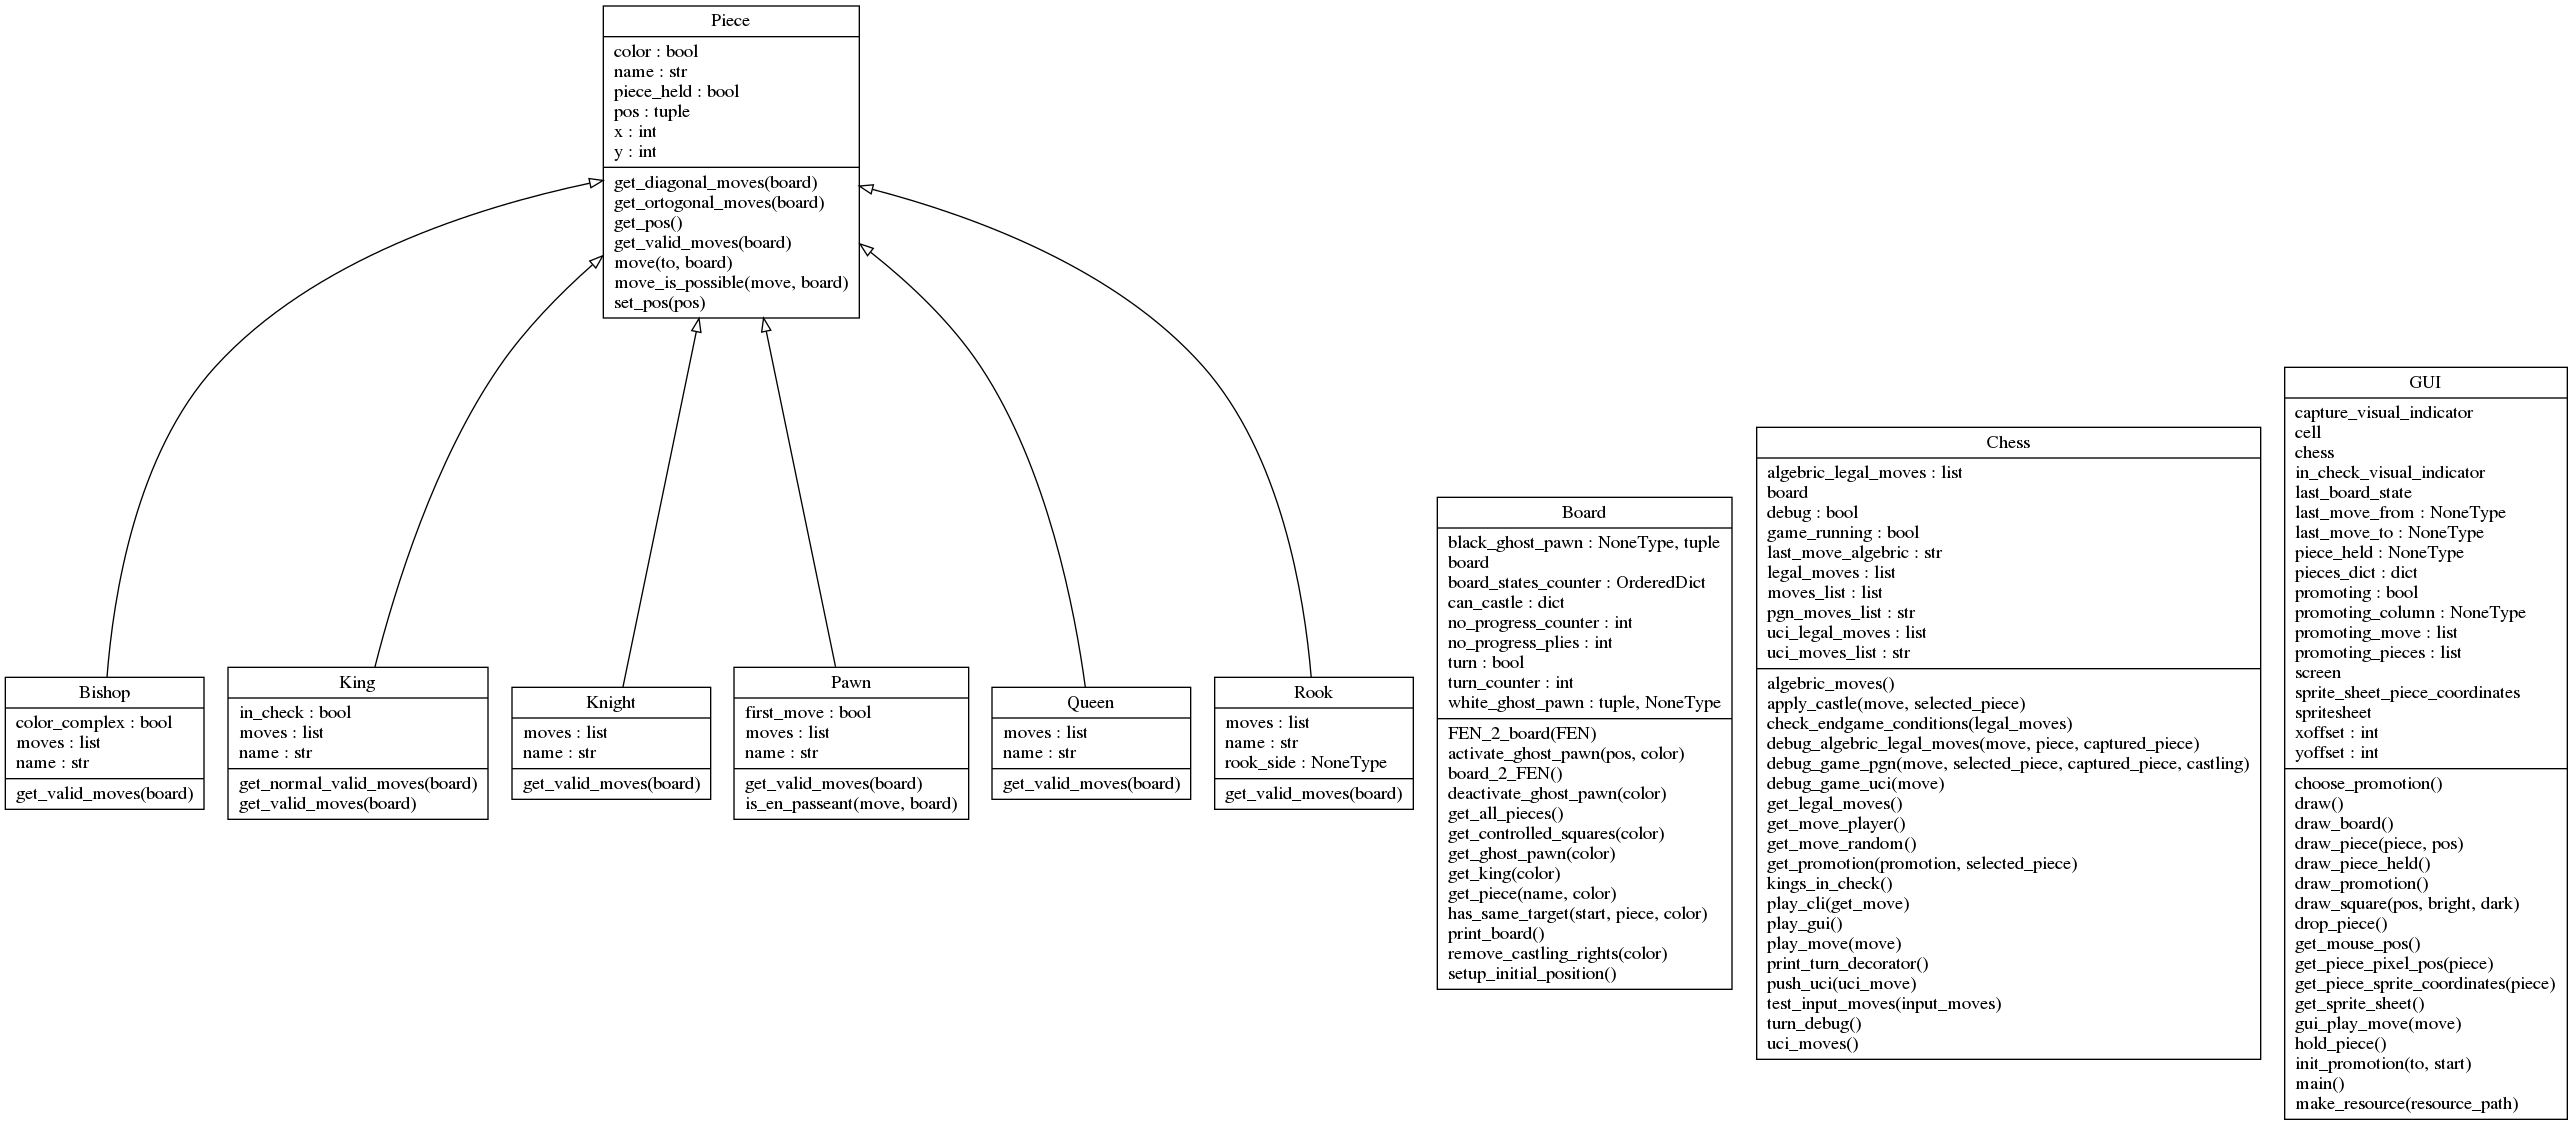
\includegraphics[scale=0.2]{fig/classes_Chess.png}
\end{figure}


\section{Testing}

\begin{table}[H]
\center
\begin{tabular}{|c|c|}
\hline
\textbf{Number of plies (half-moves)}  & \textbf{Number of possible games}  \\
\hline
  1   & 20 \\
\hline
   2  &  400 \\
\hline
  3   & 8092 \\
\hline
4  & 197,281 \\
\hline
5   & 4,865,609 \\
\hline
6   & 119,060,324 \\
\hline
\ldots & \ldots \\
\hline
10 & 69,352,859,712,417 \\
\hline
\end{tabular}
\caption{Shannon's Calculation. Obs: A turn is composed by a white move and a black move. Five plies
therefore stands for white playing three times and black two.}
\end{table}

For basic operations accuracy, it was used the Shannon Number,
which stands for all the possible moves that can be played until a certain
ply(half-move). By the limitation of the computer power avaible for our
disposal, and considering that the game was not written in a language nor
written in a way for fast computation, we could only check the precision of the
game until 5 ply, as we can see by the test log:
\begin{lstlisting}
2022-01-22 00:00:36,742 Result of possible games with 1 ply: 20/20 - OK
2022-01-22 00:00:36,742 Elapsed time in 1 ply: 00h00m00s seconds
2022-01-22 00:00:37,312 Result of possible games with 2 ply: 400/400 - OK
2022-01-22 00:00:37,312 Elapsed time in 2 ply: 00h00m00s seconds
2022-01-22 00:00:52,137 Result of possible games with 3 ply: 8902/8902 - OK
2022-01-22 00:00:52,137 Elapsed time in 3 ply: 00h00m14s seconds
2022-01-22 00:07:11,715 Result of possible games with 4 ply: 197281/197281 - OK
2022-01-22 00:07:11,715 Elapsed time in 4 ply: 00h06m19s seconds
2022-01-22 08:45:00,073 Result of possible games with 5 ply: 4865609/4865609 - OK
2022-01-22 08:45:00,073 Elapsed time in 5 ply: 08h37m48s seconds
    
\end{lstlisting}

Although this is a good signal that basic operations are working, in 5 plies we
cannot test all the complications that might arise during a chess game.

\begin{table}[h]
\center
\begin{tabular}{|c|c|c|c|c|c|c|c|c|}
\hline
\textbf{Depth}   & \textbf{Captures} & \textbf{E.P} &
\textbf{Castles} & \textbf{Promotions} & \textbf{Checks} & \textbf{Dscry
Checks} & \textbf{Dbl Checks} & \textbf{Checkmates} \\
\hline
   1  & 0 & 0 & 0 & 0 & 0 & 0 & 0 & 0 \\
\hline
   2  & 0 & 0 & 0 & 0 & 0 & 0 & 0 & 0 \\
\hline
   3  & 34 & 0 & 0 & 0 & 12 & 0 & 0 & 0 \\
\hline
   4  & 1576 & 0 & 0 & 0 & 469 & 0 & 0 & 8 \\
\hline
5  & 82,719 & 258 & 0 & 0 & 27,251 & 6 & 0 & 347 \\
\hline
\end{tabular}
\caption{Number of ``special'' moves by depth accordingly to
\url{https://www.chessprogramming.org/Perft_Results} }
\end{table}

By this table we can see that we need to concentrate our efforts in testing
Castle, Promotions, Discovery Checks and Double Checks.

One way to test them, is loading ``complex positions'', which contain it its
possibilities, castling, promotion, discovery checks and double checks, and brute forcing their
possible moves, and comparing the results with a proof table. Using the
positions recommended in \url{https://www.chessprogramming.org/Perft_Results},
we get the following result from 5 ``complex positions'':

\begin{lstlisting}
>>> $ python3 -m tests.test_brute.py (Running from top module)
2022-01-24 00:03:34,134 ----------------------------------------
2022-01-24 00:03:34,134 Initiating move generation test on depth: 2
2022-01-24 00:03:34,268 Result of possible games with 1 ply: 48/48 - OK
2022-01-24 00:03:34,268 Elapsed time in 1 ply: 00h00m00s seconds
2022-01-24 00:03:40,177 Result of possible games with 2 ply: 2039/2039 - OK
2022-01-24 00:03:40,177 Elapsed time in 2 ply: 00h00m05s seconds
2022-01-24 00:03:40,177 Total Elapsed time: (00h00m06s)
2022-01-24 00:03:40,177 -----------------------------------------
2022-01-24 00:03:40,177 ----------------------------------------
2022-01-24 00:03:40,177 Initiating move generation test on depth: 3
2022-01-24 00:03:40,195 Result of possible games with 1 ply: 14/14 - OK
2022-01-24 00:03:40,195 Elapsed time in 1 ply: 00h00m00s seconds
2022-01-24 00:03:40,454 Result of possible games with 2 ply: 191/191 - OK
2022-01-24 00:03:40,454 Elapsed time in 2 ply: 00h00m00s seconds
2022-01-24 00:03:44,350 Result of possible games with 3 ply: 2812/2812 - OK
2022-01-24 00:03:44,351 Elapsed time in 3 ply: 00h00m03s seconds
2022-01-24 00:03:44,351 Total Elapsed time: (00h00m04s)
2022-01-24 00:03:44,351 -----------------------------------------
2022-01-24 00:03:44,358 ----------------------------------------
2022-01-24 00:03:44,359 Initiating move generation test on depth: 3
2022-01-24 00:03:44,382 Result of possible games with 1 ply: 6/6 - OK
2022-01-24 00:03:44,382 Elapsed time in 1 ply: 00h00m00s seconds
2022-01-24 00:03:45,135 Result of possible games with 2 ply: 264/264 - OK
2022-01-24 00:03:45,135 Elapsed time in 2 ply: 00h00m00s seconds
2022-01-24 00:04:12,876 Result of possible games with 3 ply: 9467/9467 - OK
2022-01-24 00:04:12,876 Elapsed time in 3 ply: 00h00m27s seconds
2022-01-24 00:04:12,876 Total Elapsed time: (00h00m28s)
2022-01-24 00:04:12,876 -----------------------------------------
2022-01-24 00:04:12,881 ----------------------------------------
2022-01-24 00:04:12,881 Initiating move generation test on depth: 3
2022-01-24 00:04:12,997 Result of possible games with 1 ply: 44/44 - OK
2022-01-24 00:04:12,997 Elapsed time in 1 ply: 00h00m00s seconds
2022-01-24 00:04:17,258 Result of possible games with 2 ply: 1486/1486 - OK
2022-01-24 00:04:17,258 Elapsed time in 2 ply: 00h00m04s seconds
2022-01-24 00:07:10,379 Result of possible games with 3 ply: 62379/62379 - OK
2022-01-24 00:07:10,379 Elapsed time in 3 ply: 00h02m53s seconds
2022-01-24 00:07:10,379 Total Elapsed time: (00h02m57s)
2022-01-24 01:06:43,597 ----------------------------------------
2022-01-24 01:06:43,598 Initiating move generation test on depth: 3
2022-01-24 01:06:43,724 Result of possible games with 1 ply: 46/46 - OK
2022-01-24 01:06:43,724 Elapsed time in 1 ply: 00h00m00s seconds
2022-01-24 01:06:49,460 Result of possible games with 2 ply: 2079/2079 - OK
2022-01-24 01:06:49,460 Elapsed time in 2 ply: 00h00m05s seconds
2022-01-24 01:11:14,405 Result of possible games with 3 ply: 89890/89890 - OK
2022-01-24 01:11:14,423 Elapsed time in 3 ply: 00h04m24s seconds
2022-01-24 01:11:14,424 Total Elapsed time: (00h04m30s)
2022-01-24 01:11:14,424 -----------------------------------------
    
\end{lstlisting}

By doing these tests, we can be certain that the program is working as desired.


\pagebreak
\section{User Docs}

There are three ways to interact with this program, by directly calling their
functions in the interpreter or in a script, by calling the $play\_cli()$ or the
$play\_gui()$ functions. 

\subsection{play\_cli() and play\_gui()}

You can enter directly the CLI interface by running: $\$~python3~main.py~-cli$.
Here the program enters in a loop and continously asks moves until it reaches a
endgame condition, such as checkmate or draw.

\begin{lstlisting}

*********************************
8| r | n | b | q | k | b | n | r |
7| p | p | p | p | p | p | p | p |
6|   |   |   |   |   |   |   |   |
5|   |   |   |   |   |   |   |   |
4|   |   |   |   |   |   |   |   |
3|   |   |   |   |   |   |   |   |
2| P | P | P | P | P | P | P | P |
1| R | N | B | Q | K | B | N | R |
   a   b   c   d   e   f   g   h
*********************************

White's turn to move!

Legal moves: a2a4 a2a3 b2b4 b2b3 b1c3 b1a3 c2c4 c2c3 d2d4 d2d3 e2e4 e2e3 f2f4 f2f3 g2g4 g2g3 g1h3 g1f3 h2h4 h2h3

Move: e2e4
*********************************
8| r | n | b | q | k | b | n | r |
7| p | p | p | p | p | p | p | p |
6|   |   |   |   |   |   |   |   |
5|   |   |   |   |   |   |   |   |
4|   |   |   |   | P |   |   |   |
3|   |   |   |   |   |   |   |   |
2| P | P | P | P |   | P | P | P |
1| R | N | B | Q | K | B | N | R |
   a   b   c   d   e   f   g   h
*********************************

Black's turn to move!

Legal moves: a7a5 a7a6 b8c6 b8a6 b7b5 b7b6 c7c5 c7c6 d7d5 d7d6 e7e5 e7e6 f7f5 f7f6 g8h6 g8f6 g7g5 g7g6 h7h5 h7h6

Move:

\end{lstlisting}

You can also enter directly the GUI interface by running:
$\$~python3~main.py~-gui$. There is no time control, just dragging and dropping
pieces, and promoting pawns. The program takes care of prohibiting illegal moves
and moving enemy pieces while not your turn. Just as the play\_cli(), the game
goes on as long as it doesn't reach an endgame condition.

\begin{figure}[H]
    \center
    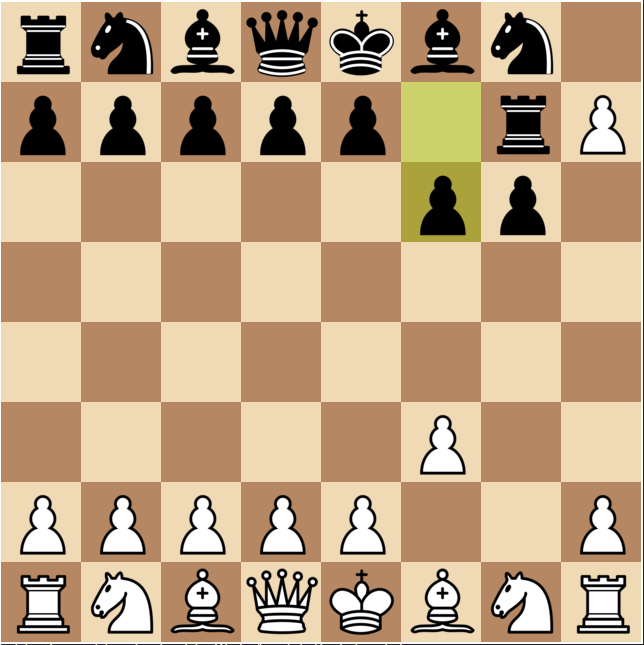
\includegraphics[scale=0.15]{{fig/pre_promotion.png}}
    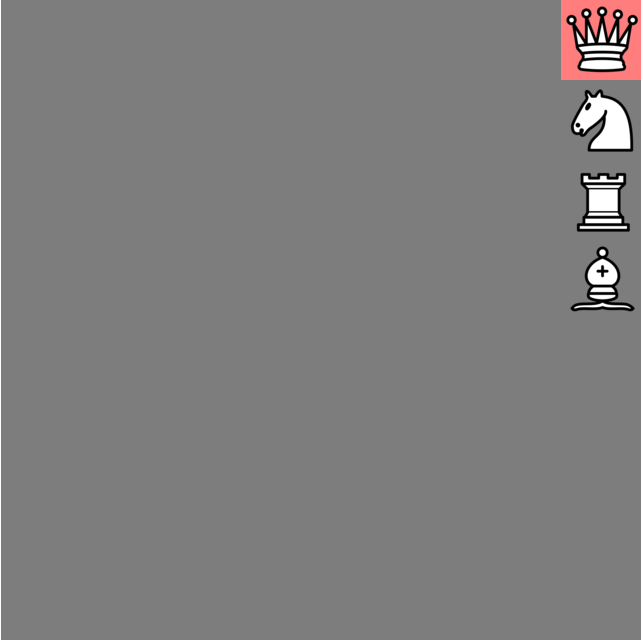
\includegraphics[scale=0.15]{{fig/promoting_pawn.png}}
    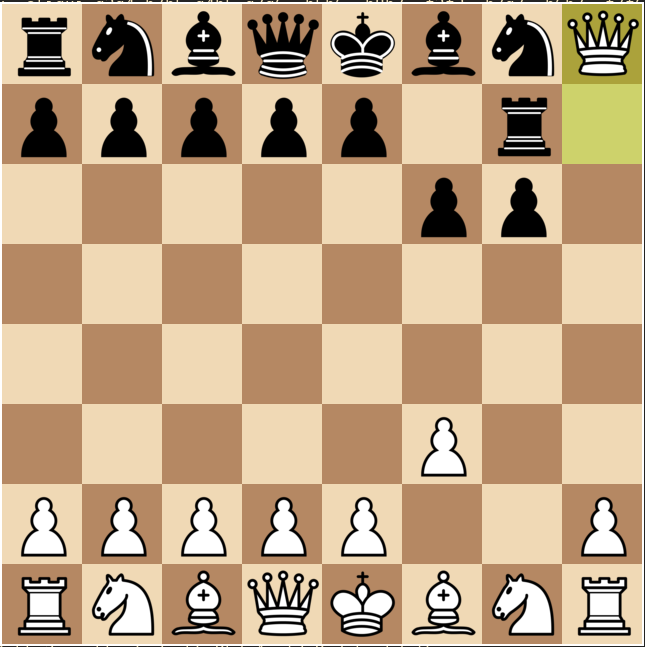
\includegraphics[scale=0.15]{{fig/promoted_pawn.png}}
    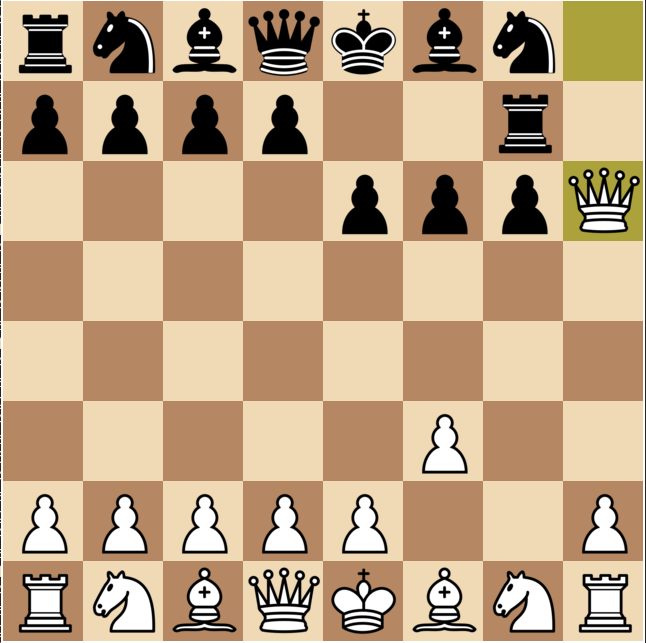
\includegraphics[scale=0.15]{{fig/queen_moving_promotion.png}}
    \caption{Overview of different states of the game while in GUI. With a
    Pawn promoting to a Queen.}
\end{figure}

\subsection{Other Uses}

By importing the mychess module, we open other possibilities, like loading a
position and playing it from there.



\end{document}

